\chapter{Stage 03: labels and evidence cards}
\label{ch:stage03}

Stage~03 produces three things for every patch (the three orange boxes in your workflow figure): the pair of colour images (Chapter~\ref{ch:stage02}), the \textbf{automatic label}, and the \textbf{evidence card}. This chapter explains the last two, because every result in the report depends on them.

\section{The automatic label}
\label{sec:labels}

\subsection{The rule}

Notebook 01, cell 17, assigns \texttt{candidate\_class} from each patch's mean NDVI change $\Delta$ and the 15th and 85th percentiles of $\Delta$ over the 1,200-patch pool, $q_{15} = -0.0377$ and $q_{85} = +0.0031$:
\begin{equation}
\text{class} =
\begin{cases}
\text{uncertain} & \text{masked fraction} > 0.15 \text{ in either year,}\\
\text{decline} & \Delta \le q_{15},\\
\text{increase} & \Delta \ge q_{85},\\
\text{stable} & |\Delta| < 0.05,\\
\text{uncertain} & \text{otherwise.}
\end{cases}
\label{eq:labelrule}
\end{equation}
Uncertain patches were never sampled. Because both percentiles lie inside $\pm0.05$, every unmasked patch between $q_{15}$ and $q_{85}$ is labelled stable, and the last ``uncertain'' case never happens for this pool. In practice the rule is: \emph{bottom 15\,\% of NDVI change is decline, top 15\,\% is increase, the rest is stable}.

\begin{whybox}
The roadmap (Section~6) says to ``begin with region-specific quantiles rather than claiming universal ecological thresholds''. Percentiles guarantee enough examples of each class even in a year with little real change, and they avoid borrowing thresholds from studies of other forests.
\end{whybox}

\begin{figure}[H]
\centering
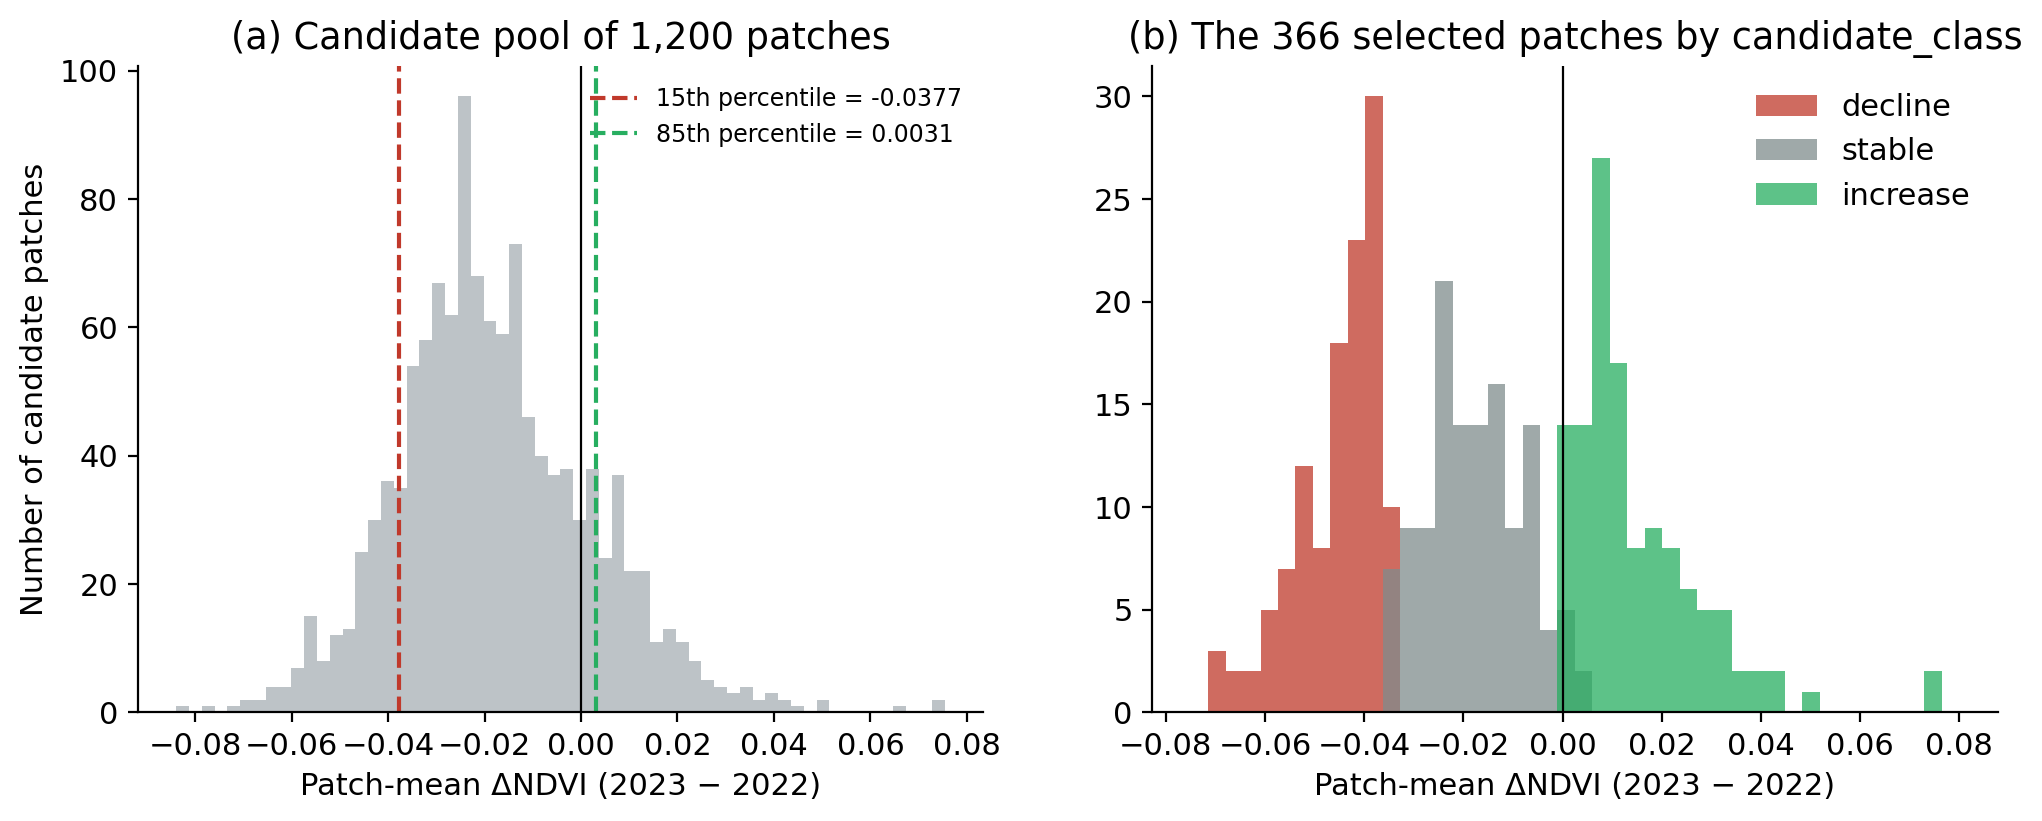
\includegraphics[width=\textwidth]{figures/fig_ndvi_labels.png}
\caption{(a) Patch-mean \dndvi{} over the 1,200-patch pool with the 15th and 85th percentiles; most patches lost a little greenness. (b) \dndvi{} of the 366 selected patches by label. From \file{data/raw_metadata/}.}
\label{fig:ndvilabels}
\end{figure}

\subsection{How the 366 patches were chosen}

The first 300 patches (100 per class) were selected in the parent repository. Notebook 01, cell 17, then added up to 25 per class from the rest of the pool, keeping new centres at least 960\,m (1.5 patch widths) from all existing ones; only 22 decline candidates passed that distance filter. This gave 372 patches. Six had incomplete exports and were moved to \file{data/outcasts/}, leaving \textbf{366: 120 decline, 124 stable, 122 increase}.

\begin{watchout}
For the 72 added patches the percentiles were recomputed on the \emph{remaining} pool, so their cut-offs differ slightly from those of the first 300. The class ranges therefore overlap a little: decline patches reach $\Delta = -0.034$ while stable patches go down to $-0.036$, and increase patches go down to $-0.001$ while stable patches reach $+0.003$ (Figure~\ref{fig:ndvilabels}b). The labels are almost, but not exactly, a function of $\Delta$.
\end{watchout}

\subsection{What the labels really mean}

\begin{plainwords}
The whole region became slightly less green between the two years (mean \dndvi{} $= -0.016$, standard deviation 0.027). So the percentile rule calls ``increase'' anything in the greenest 15\,\%, even if it barely changed: an increase patch has \dndvi{} anywhere from $-0.001$ to $+0.075$, and half of them changed by less than 0.011. ``Decline'' means ``among the 15\,\% that lost the most greenness'', here a drop of about 0.034 to 0.071. ``Stable'' means ``in between''. Only 34 of the 366 patches changed NDVI by 0.05 or more in either direction.
\end{plainwords}

The labels are \textbf{relative ranks within this region and pair of years}, not absolute ecological states. That is acceptable for a benchmark if you say it clearly. It is wrong to call increase patches ``recovering forest'' or decline patches ``degraded'' or ``deforested''.

\section{The human check}
\label{sec:humanlabels}

The roadmap asked for manual validation and an independent audit. What was done:

\begin{itemize}
  \item \textbf{Pilot, early September}: 36 patches reviewed by a person; automatic and human labels agreed on 17 of 36 (47\,\%) (\file{summary.txt}).
  \item \textbf{Final dataset}: 19 patches carry a \texttt{reference\_class} (13 train, 3 development, 3 test). The automatic label agrees on \textbf{8 of 19 (42\,\%; 95\,\% interval 23--64\,\%)} (\file{results/preflight_report.json}). The other pilot patches are kept in \file{data/pilot_reference/}.
  \item No second reviewer and no expert audit.
\end{itemize}

\begin{table}[H]
\centering
\caption{Automatic label against human label for the 19 patches in the final dataset (rows: automatic; columns: human).}
\label{tab:humanagree}
\begin{tabular}{lccc|c}
\toprule
 & human decline & human stable & human increase & total \\
\midrule
auto decline & 3 & 2 & 1 & 6 \\
auto stable & 0 & 2 & 1 & 3 \\
auto increase & 4 & 3 & 3 & 10 \\
\midrule
total & 7 & 7 & 5 & 19 \\
\bottomrule
\end{tabular}
\end{table}

Some disagreements are large: p01350 lost 0.040 NDVI but the person called it ``increase''; p03545 and p04416 gained NDVI but were called ``decline''. The person presumably judged the colour images, where changes this small are hard to see, while the rule reads a number the eye cannot see. Neither is ``truth''. Only 3 of the 10 automatic \texttt{increase} patches that were checked were confirmed, so \texttt{increase} is the least reliable class.

\begin{foryourreport}
The repository does not record how the human labels were made. Write down your actual procedure (who looked, at what images, with which instructions) and report it in Methods. Report the agreement as ``8 of 19 (42\,\%)'' with the interval, and call the automatic labels ``operational reference labels'' or ``automatic labels'', not ``ground truth''.
\end{foryourreport}

\section{The evidence card}
\label{sec:card}

\subsection{Two versions of the text}

\begin{enumerate}
  \item \textbf{Version 1} (\file{scripts/03_build_dataset.py}) tried to have a local language model (through Ollama) write an explanation for each patch. Ollama was not running, so all 366 fell back to a fixed template filled with numbers (\file{results/preflight_report.json}: ``ollama=0, fallback=366''). These texts survive only in \file{dataset_old.jsonl}.
  \item \textbf{Version 2} (\file{scripts/build_extensive_jsonl.py}, \texttt{enrich\_row} in \file{src/extensive_descriptions.py}) replaced them with text \emph{computed from the rasters}. Every record in the final \file{dataset.jsonl} has \texttt{explanation\_source = raster\_analysis\_v2}, and all 366 texts are different.
\end{enumerate}

\begin{newinfo}
Your current draft says that ``all narrative explanations are just templates, because no language model based explanation was obtained''. That sentence came from the rewrite I gave you earlier, and it is wrong for the final dataset: the stored text is a rule-based narrative computed from each patch's rasters. What is true is that \emph{no language model wrote it}. Correct the sentence (Chapter~\ref{ch:draft}).
\end{newinfo}

\subsection{How version 2 is built}

For each patch, \texttt{enrich\_row}:
\begin{enumerate}
  \item reads the colour GeoTIFFs and measures brightness and ``green cover'' (the share of pixels where green is the largest channel);
  \item loads the 512\,$\times$\,512 arrays of indices, radar and \dndvi{} and computes means, percentiles and the share of pixels that fell below $-0.05$ or rose above $+0.05$;
  \item takes rainfall, ERA5-Land and terrain values from the record;
  \item turns numbers into words with simple rules (Table~\ref{tab:inferrules});
  \item assembles a narrative and the model prompt, \texttt{condition\_c\_user\_prompt}.
\end{enumerate}

\begin{table}[H]
\centering
\caption{Rules that convert measurements into the words on the card (\texttt{\_infer\_signals} in \file{src/extensive_descriptions.py}).}
\label{tab:inferrules}
\small
\begin{tabularx}{\textwidth}{lY}
\toprule
Field & Rule \\
\midrule
vegetation\_trend & strong\_decline if \dndvi{} $\le -0.04$ and at least 8\,\% of pixels dropped by more than 0.05; moderate\_decline if \dndvi{} $\le -0.02$; greening if $\ge +0.02$ and at least 8\,\% rose by more than 0.05; slight\_greening if $\ge +0.01$; otherwise stable \\
fire\_burn\_likelihood & elevated\_burn\_signal if the NBR mask exceeds the NDVI mask by 2 points and \dnbr{} $< -0.02$; deforestation\_pattern if the NDVI mask exceeds 2\,\% and boxes exist; otherwise low \\
candidate\_class\_consistency & agrees if the label and the trend point the same way; spatial\_anomaly if the label is stable but boxes exist; otherwise partial\_mismatch \\
sar\_evidence\_strength & notable\_backscatter\_shift if $|\Delta\mathrm{VV}| \ge 0.8$\,dB, otherwise secondary \\
climate\_evidence\_strength & drier\_second\_window if rainfall fell by at least 25\,mm; wetter if it rose by at least 25\,mm; otherwise neutral \\
terrain\_context & steep\_terrain if slope $\ge 12^\circ$, otherwise gentle\_terrain \\
\bottomrule
\end{tabularx}
\end{table}

\subsection{A real card, with the line that matters}

This is the text that Qwen2-VL-2B and LLaVA received in Track~A for test patch p00575 (gold label \texttt{decline}):

\begin{tcolorbox}[colback=gray!4,colframe=gray!50,fontupper=\scriptsize\ttfamily,breakable]
Task: ground\_forest\_disturbance\_in\_spectral\_evidence\\
Condition C evidence (measured on disk, analysis v2):\\
T0 (2022) terrain RGB (65$\times$69 native, stretched for display): brightness=0.169, green-cover=0.74, uniform illumination; canopy-green dominates. T1 (2023) terrain RGB (65$\times$69 native, stretched for display): brightness=0.198, green-cover=0.42, uniform illumination; mixed canopy and non-photosynthetic pixels. Brightness change T1$-$T0=+0.0292 on natural-color chips.\\
On the 512$\times$512 aligned stack, mean NDVI 0.6248$\rightarrow$0.5752 ($\Delta$=-0.0496), NBR 0.3106$\rightarrow$0.3135 ($\Delta$=+0.0029), EVI $\Delta$=-0.0040, NDMI $\Delta$=-0.0070. $\Delta$NDVI raster: mean=-0.04966, 48.9\% pixels below $-$0.05, 0.4\% above +0.05; $\Delta$NBR raster mean=0.0029.\\
SAR (512$\times$512 means): VV -8.624$\rightarrow$-8.839 dB ($\Delta$-0.22), VH -14.322$\rightarrow$-14.734 dB ($\Delta$-0.41); interpreted as secondary.\\
CHIRPS Jan--Feb total 72.5$\rightarrow$25.4 mm ($\Delta$-47.1 mm, drier\_second\_window). ERA5-Land anomalies: temperature -1.50$\rightarrow$+1.08 \textdegree C, soil moisture +0.027$\rightarrow$-0.048 vs 2015--2021 climatology.\\
NASADEM at patch center: 834 m, slope 5.1\textdegree, aspect 160\textdegree{} (gentle\_terrain).\\
No Otsu boxes (NDVI mask active on 21.7\% of pixels, NBR mask on 3.5\%).\\
\colorbox{red!20}{Inference for p00575: vegetation\_trend=strong\_decline,}\\
\colorbox{red!20}{burn/deforestation cue=low, candidate\_class=decline}\\
\colorbox{red!20}{(agrees with spectra/boxes).}\\
Respond with class (stable/decline/increase) and a short grounded explanation.
\end{tcolorbox}

The highlighted line is the \textbf{pipeline's summary line}. \texttt{synthesize\_narrative} in \file{src/extensive_descriptions.py} builds every card from seven pieces, and the last piece, \texttt{conclusion}, is this summary. It was written for a human reader of the card, and it states \texttt{candidate\_class}, the same field that is used as the gold label. Because it is part of \texttt{condition\_c\_user\_prompt}, every full card given to a model contains the answer.

\begin{plainwords}
This is not a scandal; it is a fact about the input that must be stated. A model shown the full card can get a patch right by reading the label, by reading the numbers, by looking at the images, or by a mixture. Track~A's numbers therefore measure ``how well a model uses the complete card''. Chapter~\ref{ch:trackA} explains what the project did to separate these, and what it could not separate.
\end{plainwords}

\section{The card does not always agree with the label}

The card's \texttt{vegetation\_trend} words use a different rule from the label (Table~\ref{tab:inferrules}). Comparing the two over all 366 patches (Figure~\ref{fig:labeltrend}):
\begin{itemize}
  \item 258 patches agree and \textbf{108 disagree} (``partial\_mismatch'').
  \item Every \texttt{decline} patch has a declining trend (54 strong, 66 moderate).
  \item \textbf{61 of 122 \texttt{increase} patches} have the trend ``stable''.
  \item 47 of 124 \texttt{stable} patches have the trend ``moderate\_decline''.
\end{itemize}

\begin{figure}[H]
\centering
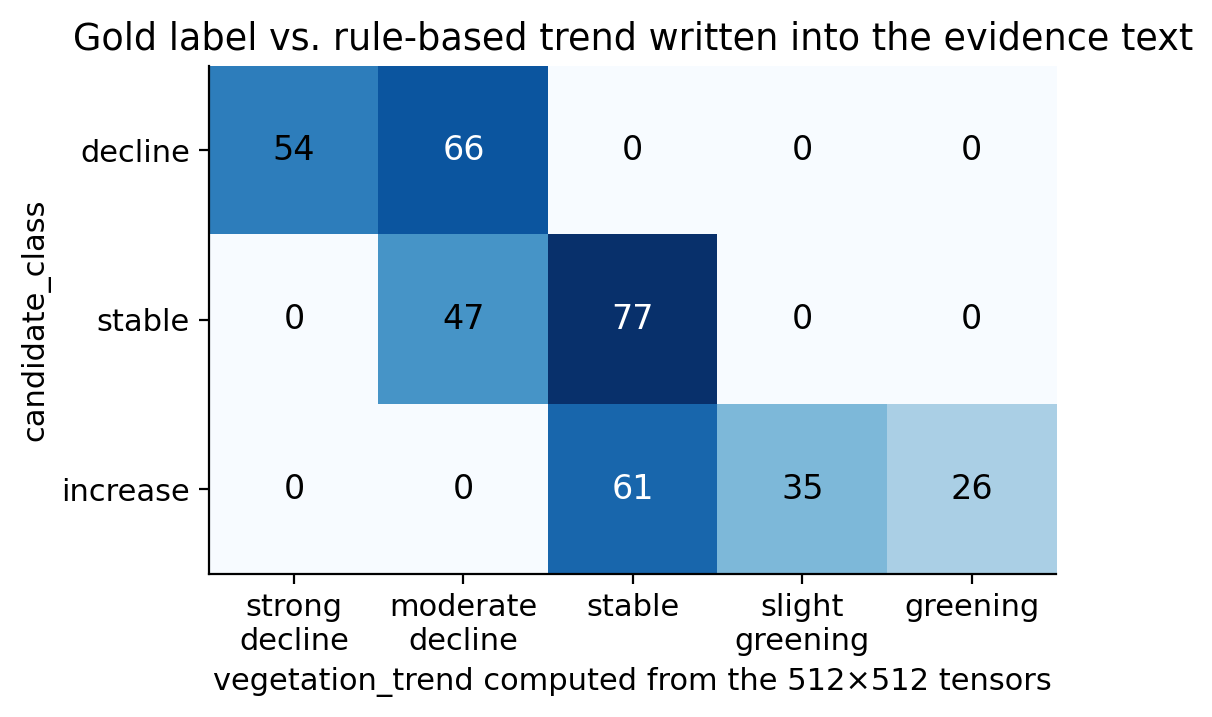
\includegraphics[width=0.78\textwidth]{figures/fig_label_vs_trend.png}
\caption{Gold label against the rule-based trend written into the evidence card (\file{dataset.jsonl}).}
\label{fig:labeltrend}
\end{figure}

The two disagree because they apply different thresholds to different numbers: the label uses the region's percentiles ($-0.038$ and $+0.003$) of the Earth Engine patch mean; the trend uses fixed cut-offs ($\pm0.02$ and $+0.01$) on the padded canvas mean. A model shown the full card can therefore receive two signals that point different ways: the trend word says ``stable'' while the summary line says \texttt{candidate\_class=increase}.

\section{The padding bias in the card's numbers}
\label{sec:padbias}

The means on the card are taken over the whole 512\,$\times$\,512 canvas, padding included (Chapter~\ref{ch:stage02}). If a fraction $f$ of the canvas is zero padding,
\begin{equation}
\bar{x}_{\text{reported}} = (1-f)\,\bar{x}_{\text{true}} + f\cdot 0 = (1-f)\,\bar{x}_{\text{true}} .
\end{equation}
For a normal 65-row chip, $1-f \approx 0.93$, so the NDVI on the card is about 7--8\,\% too low; averaged over all patches, the card's NDVI is 0.92 times the Earth Engine mean. For the clipped edge patch p00052 the factor is about 0.43, and its NDVI appears as 0.31 instead of about 0.7. Radar values (negative decibels) are pulled towards 0\,dB.

\begin{figure}[H]
\centering
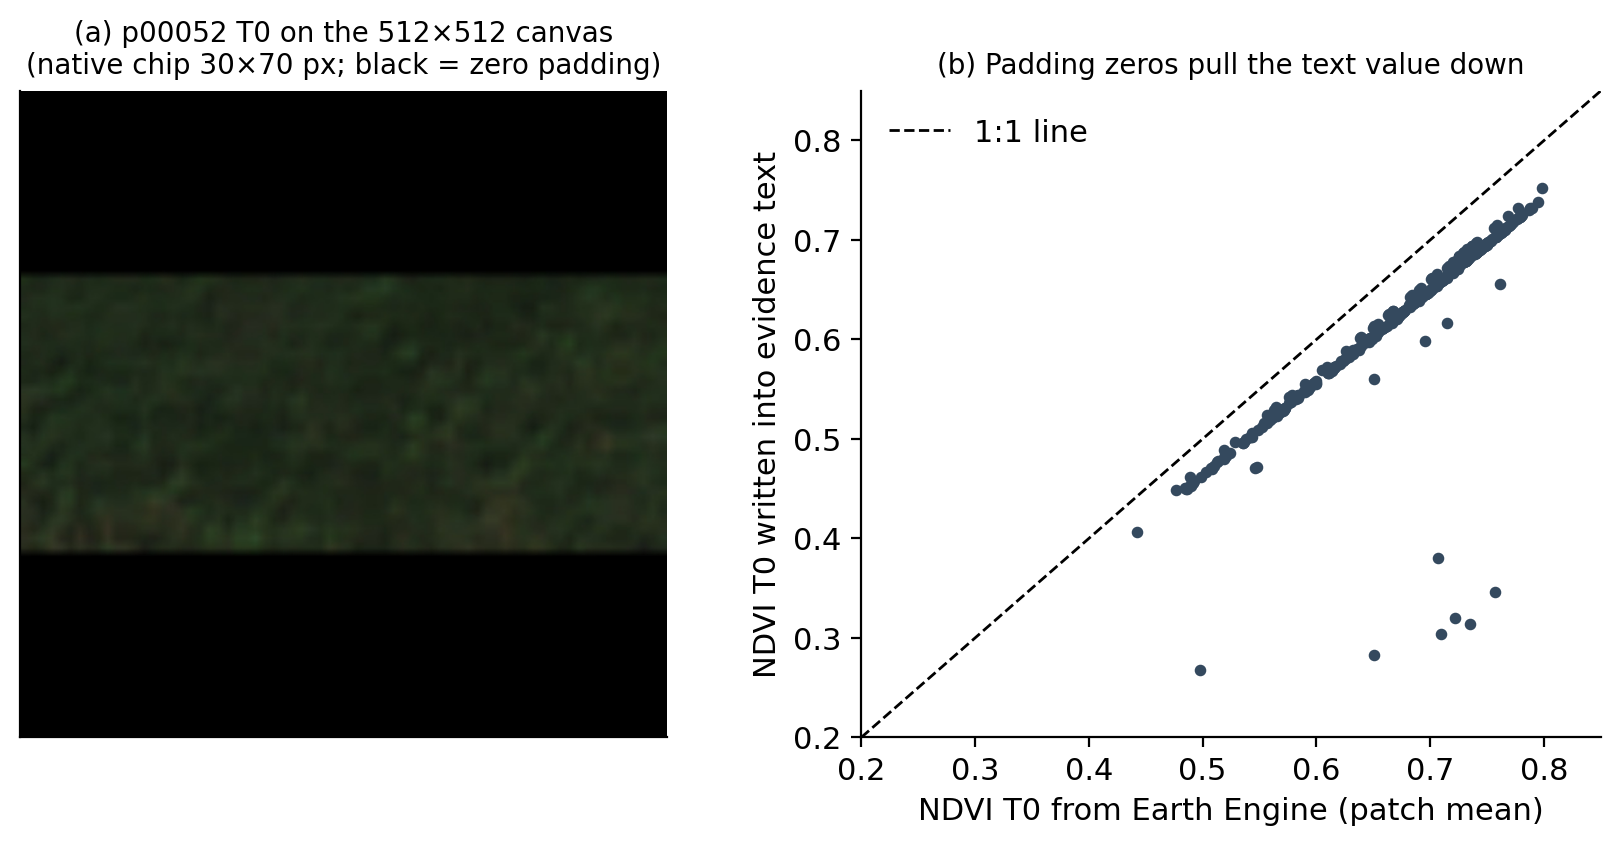
\includegraphics[width=0.9\textwidth]{figures/fig_padding_bias.png}
\caption{(a) An edge patch on the canvas: most of the image is padding. (b) NDVI written on the card against the Earth Engine patch mean; points below the 1:1 line are biased low, and the isolated low points are clipped edge patches.}
\label{fig:padbias}
\end{figure}

The \emph{changes} are scaled by the same factor, so their sign is right and they correlate 0.995 with the Earth Engine values, but their size is understated. The fix is simple for future work: pad the arrays with ``not a number'' instead of 0, or compute statistics on the original chip.

\begin{foryourreport}
In ``Change Evidence and Labelling'' (about 600 words):
\begin{itemize}
  \item The label rule as an equation (Equation~\ref{eq:labelrule}) and the two percentile values; say that the last case never occurs.
  \item The sampling (300 + 72, 960\,m spacing, 6 incomplete, final 120/124/122) and the slight class overlap.
  \item What the classes mean: relative ranks, small changes, 34 patches with $|\Delta| \ge 0.05$.
  \item The human check (8 of 19) and your procedure.
  \item The card: what it lists, that it was computed from the rasters (version 2), that its last line repeats \texttt{candidate\_class}, and that its trend words disagree with the label on 108 patches.
  \item The padding bias in one or two sentences (here or in Limitations).
\end{itemize}
\end{foryourreport}

\begin{selfcheck}
\begin{enumerate}
  \item State the labelling rule in one sentence without the equation.
  \item Why can a patch whose NDVI fell slightly be labelled \texttt{increase}?
  \item What are the two versions of the card text, and which one is in the final dataset?
  \item What is the summary line, and why does it matter for Track~A?
  \item Why do the card's trend words disagree with the label for 108 patches?
  \item Why is the NDVI written on the card about 8\,\% too low?
\end{enumerate}
\end{selfcheck}
